% !TEX program = xelatex
% 形态 B（消元式单扇区）的数学原理
% 编译：xelatex MATHEMATICS.tex（需 ctexart + Noto CJK；跑两遍生成目录/引用）
\documentclass[11pt,a4paper]{ctexart}

\usepackage[margin=2.4cm]{geometry}
\usepackage{amsmath,amssymb,mathtools}
\usepackage{booktabs}
\usepackage{graphicx}
\usepackage{xcolor}
\usepackage[colorlinks=true,linkcolor=blue!60!black,urlcolor=blue!60!black]{hyperref}

% ---- 生成元记号 ----
\newcommand{\ab}{\bar a}          % IF bar
\newcommand{\xb}{\bar x}          % IMP bar
\newcommand{\Pf}{\operatorname{Pf}}
\newcommand{\Tr}{\operatorname{Tr}}
\newcommand{\tr}{\operatorname{tr}}
\newcommand{\antisym}{\operatorname{antisym}}
\newcommand{\Deff}{D}             % Δ_eff 的反对称多项式形式
\newcommand{\Pelim}{P_{\mathrm{elim}}}

\title{\textbf{形态 B（消元式单扇区）的数学原理}\\
\large ——IF 变量的精确高斯消元与 GTEMPO GrassmannMPS 实现}
\author{benchmark/exactif 工作笔记}
\date{2026 年 11 月}

\begin{document}
\maketitle

\begin{abstract}
本文给出形态 B 表示的完整数学推导：以 IFGTEMPO 的两扇区 Grassmann
路径积分为起点，把 bath 影响 IF 的生成元通过\textbf{带线性源的精确
高斯积分}积掉，得到只剩一套杂质轨迹变量、由有效双线性核
$\Deff[\lambda,\lambda']$ 与归一化常数 $\nu\Pf(G)$ 描述的等价表示；
进而说明它与 GTEMPO pair 收缩机制（隐式 resolution 测度、幂零反测度、
graded 读出符号）的逐条数学对接。实现分布于
\texttt{form\_b/formb\_dense.jl}（稠密系数级验证，保留）与
\texttt{src/FormB.jl}（GTEMPO GMPS 移植，已于 2026-11-07 删除）；文中每条公式均标注了
验证位置（\S\ref{sec:verify}）。
\end{abstract}

\tableofcontents

% ============================================================================
\section{设定：离散 Trotter 链与两扇区变量}
% ============================================================================

\subsection{算符链与迹保持}

总 Hamiltonian 分解为杂质踢与二次胞（$H_Q$ 的杂质对角为零，杂质能级
归踢算符携带）：
\begin{equation}
H = H_{\mathrm{imp}} + H_Q,\qquad
A(\ell) = e^{-i\ell H_{\mathrm{imp}}},\qquad
Q(c) = e^{-icH_Q}.
\end{equation}
Trotter 调度（order $1/2/4$，\texttt{trotter\_schedule}）给出胞长
$c_1,\dots,c_{n_c}$ 与链节长 $\ell_1,\dots,\ell_{n_c+1}$：order~2 为
Strang 合并半步 $\ell = (\delta t/2,\delta t,\dots,\delta t,\delta t/2)$；
order~4 为 Suzuki $S_2(a\delta t)^2 S_2(b\delta t)$、$2a+b=1$（
$a=(2-2^{1/3})^{-1}$，$b=1-2a<0$），合并内层 $\ell=(a+b)/2$ 可为负。
离散链（矩阵积右端先作用）：
\begin{equation}
U \;=\; A(\ell_{n_c+1})\,Q(c_{n_c})\,A(\ell_{n_c})\cdots Q(c_1)\,A(\ell_1),
\qquad
\rho^{\mathrm{disc}}_{\mathrm{imp}}
=\Tr_B\!\big[U(\rho_0\otimes\rho_B)U^\dagger\big].
\label{eq:chain}
\end{equation}
实时 Keldysh 围道：前向支携带 $U$、后向支携带 $U^\dagger$。
所有因子幺正，故迹保持
\begin{equation}
Z \;=\; \tr\rho^{\mathrm{disc}}_{\mathrm{imp}} = \tr\rho_0 = 1,
\end{equation}
对任意参数与任意 order 成立——这是区分表示结构正确性的最锐利证书。

\subsection{变量与 lattice}

每个 $U_{\mathrm{imp}}$--$U_{\mathrm{bath}}$ 接口插入一个 Grassmann
恒等 resolution $1=\int d\bar x\,dx\;e^{-\bar xx}\,|x\rangle\langle\bar x|$。
接口 $t$（$t=1..n_c$）的生成元分两扇区，每 flavor $8$ 个 site
（\texttt{timelocallattice} 序）：
\begin{equation}
\big(\ab_t^{+},\,x_t^{+},\,\xb_t^{+},\,a_t^{+},\;\;
     \ab_t^{-},\,x_t^{-},\,\xb_t^{-},\,a_t^{-}\big),
\label{eq:layout}
\end{equation}
\begin{itemize}
\item \textbf{IF 变量} $a,\ab$（bath 响应）：$G$ 矩阵槽位序为
  $\mathrm{slot}\,0,1,2,3=(\ab_t^{+},a_t^{+},\ab_t^{-},a_t^{-})$，
  一维指标 $\mathrm{flat}=4(t{-}1)+\mathrm{slot}+1$（1-based）；
\item \textbf{IMP 轨迹变量} $x,\xb$：$x_t^{\pm}$（eta 腿）是链节
  $\ell_{t+1}$ 的输入 ket，$\xb_t^{\pm}$（bar 腿）是 $\ell_t$ 的输出 bra；
\item layer $0$：$(\xb_0^{+},x_0^{+},\xb_0^{-},x_0^{-})$，初态核
  $\langle\xb_0^{+}|\rho_0|x_0^{-}\rangle$；
\item layer $N{+}1$（开放腿）：$\xb_{N+1}^{+},\,x_{N+1}^{-}$，
  保留为 $\rho(T)$ 的读出腿。
\end{itemize}
关键布局性质：相邻 site 恰为一个恒等 resolution 的 (bar, eta) 对，
使每接口的交叉测度天然落在 GTEMPO 的 pair 上（\S\ref{sec:pair}）。

% ============================================================================
\section{两扇区多项式}
% ============================================================================

两扇区路径积分的全部内容为
\begin{equation}
P(a,x)\;=\;\nu\,e^{\frac12 a^{T}Ga}\;
   \prod_{t=1}^{n_c} M_t\;\cdot\;M_0\;\cdot\;K[x],
\qquad
M_t = e^{-\ab_t^{+}x_t^{+}-\xb_t^{+}a_t^{+}
                  -\ab_t^{-}x_t^{-}-\xb_t^{-}a_t^{-}},
\label{eq:twosector}
\end{equation}
各因子的物理来源：

\begin{enumerate}
\item \textbf{IF Gaussian}
  $e^{\frac12 a^TGa}=e^{\sum_{i<j}G_{ij}a_ia_j}$：$G$ 为反对称 IF 系数
  矩阵（\texttt{influence\_matrix\_G}）——bath 围道大矩阵
  $\mathsf A=\begin{pmatrix}E&C\\-C^{T}&B\end{pmatrix}$（bath 生成元、
  热核、逐 pair 恒等测度、反周期 trace 边界）对 bath 块的 Schur 补
  $G=\antisym(E+CB^{-1}C^{T})$，其元素即论文六类相关函数族；
  $\nu=Z_N/Z$ 为传播后热 bath 迹对未传播迹之比。
\item \textbf{接口交叉测度} $M_t$：恒等 resolution 的 ket 变量归左核、
  bra 变量归右核，故测度把 IF 与 IMP 扇区\textbf{交叉}配对——
  ``两扇区''结构的来源（IFGTEMPO 推导文档 \S3、\S9）。
\item \textbf{layer 0 测度}
  $M_0=e^{-\xb_0^{+}x_0^{+}-\xb_0^{-}x_0^{-}}$。
\item \textbf{$K[x]$}：踢核
  $\langle\xb_t^{\pm}|A(\ell_t)|x_{t-1}^{\pm}\rangle$（前向对角
  $e^{-i\ell\epsilon}$、后向 $A^\dagger$）+ 初态核。单项式符号配方
  $\mathrm{coeff}(\mathrm{bra},\mathrm{ket})
  =(-1)^{C(\mathrm{ket},2)}\,K[\mathrm{bra}{+}1,\mathrm{ket}{+}1]$，
  $C(n,2)=n(n{-}1)/2$ 为双占据符号，local 序 (bar$\dots$, eta$\dots$)。
\end{enumerate}

物理量读出：\textbf{开放核}
$\langle\xb_{N+1}^{+}|\rho(T)|x_{N+1}^{-}\rangle$（积掉全部内部变量、
保留开放腿，系数按配方逆映射回矩阵）；\textbf{迹}按反周期边界
\begin{equation}
\Tr\rho=\int d\bar x\,dx\;e^{-\bar xx}\,
\langle-\bar x|\rho|x\rangle ,
\label{eq:trace}
\end{equation}
把 $\langle\bar x|\to\langle-\bar x|$ 的翻转并入闭合符号后即闭合因子
$(1+\xb_{N+1}^{+}x_{N+1}^{-})$，系数 $+1$（取 $-1$ 为周期迹，$Z\ne1$，
已被证书排除）。

% ============================================================================
\section{消元：IF 变量的精确高斯积分}
\label{sec:elim}
% ============================================================================

\subsection{源嵌入}

全部含 $a$ 的指数项集中，接口测度成为 IF 生成元上的\textbf{线性源}：
\begin{equation}
\frac12 a^{T}Ga+\sum_t\big(-\ab_t x_t-\xb_t a_t\big)
 =\frac12 a^{T}Ga+j^{T}a,
\qquad
j_i=-\,\theta_{\lambda(i)} ,
\end{equation}
即 IF bar slot（$\ab_t^{\pm}$）的 partner 为 IMP eta 腿 $x_t^{\pm}$、
IF eta slot（$a_t^{\pm}$）的 partner 为 IMP bar 腿 $\xb_t^{\pm}$
（bar$\leftrightarrow$eta 交叉）。

\subsection{高斯恒等式}

\begin{equation}
\boxed{\;\int \mathcal D a\,
\exp\!\Big(\tfrac12 a^{T}Ga+j^{T}a\Big)
=\Pf(G)\,\exp\!\Big(-\tfrac12 j^{T}G^{-1}j\Big)\;}
\label{eq:gauss}
\end{equation}
配方：$-\tfrac12\xi A\xi+\eta\xi
=-\tfrac12(\xi-\eta A^{-1})A(\xi-\eta A^{-1})+\tfrac12\eta A^{-1}\eta$，
Grassmann 积分的平移不变性把平方项积出 $\Pf$。$n{=}2$ 直算核验：
$\int e^{A_{12}a_1a_2+j_1a_1+j_2a_2}=A_{12}+j_1j_2$，与公式一致。

\subsection{$\Deff$ 的显式形式}

代入 $j_i=-\theta_{\lambda(i)}$ 并取递增 monomial
$\theta_\lambda\theta_{\lambda'}$（$\lambda<\lambda'$ 按 site 序；
$i=\mathrm{slot}(\lambda)$、$k=\mathrm{slot}(\lambda')$）的系数：
$(i,k)$ 项贡献 $-\tfrac12G^{-1}[i,k]$，$(k,i)$ 项经
$\theta_{\lambda'}\theta_\lambda=-\theta_\lambda\theta_{\lambda'}$
贡献 $+\tfrac12G^{-1}[k,i]$，合计
\begin{equation}
\boxed{\;\Deff[\lambda,\lambda']
 =-\tfrac12\big(G^{-1}[i,k]-G^{-1}[k,i]\big)\;}
\qquad(\lambda<\lambda')
\label{eq:Deff}
\end{equation}
只依赖 $G^{-1}$ 的\textbf{反对称部分}——对称部分因 $\theta$ 反对易
自动消失。此即总览中 $\Delta_{\mathrm{eff}}=-\tfrac12P^{T}G^{-1}P$
的反对称多项式形式（$P$ 为接口配对映射）。

\subsection{消元多项式及其性质}

\begin{equation}
\Pelim(x)\;=\;\nu\Pf(G)\;
   e^{\sum_{\lambda<\lambda'}\Deff[\lambda,\lambda']\theta_\lambda\theta_{\lambda'}}\;
   K[x]\;M_0 .
\label{eq:pelim}
\end{equation}
\begin{enumerate}
\item \textbf{精确恒等式}：$\int\mathcal Da\,P=\Pelim$，无近似、无信息
  损失；全部接口测度被吸收，消元表示中内部接口不得再出现任何测度。
\item $\Deff$ 只作用在接口轨迹腿上（layer 0 / 开放腿无源，对应行列全零）。
\item $\Deff$ 稠密、非局域（$G^{-1}$ 所致）——与 QuAPI 冻结核
  $\Delta t$ 的稀疏时序结构不同，二者是同一离散链的不同多项式实现，
  不可逐元素互换。骨架测度 $-\ab x$ 的吸收表现为 $\Deff$ 在同接口相邻
  slot 对上的测度块（$\approx-\tfrac12$）。
\item 归一化 $\nu\Pf(G)$ 替代精确核 prefactor。
\end{enumerate}

\subsection{收缩语义：投影积分与迹闭合}

稠密表示的全收缩 = 逐生成器提系数（$\int d\theta\,\theta f\to f$，
顺序任意）。每个 monomial 中每个生成元至多出现一次，故该投影与次序
无关、无定向符号——测度权重已全部显式在多项式因子里，与 GTEMPO pair
sweep 的逐 pair 带权规则 $f_0-f_{be}$ 是同一运算的两种分布方式
（\S\ref{sec:pair}）。迹闭合：取闭合因子 $(1+\xb^{+}x^{-})$ 后，
全投影给出 $Z=\rho_{00}+\rho_{11}=\tr\rho(T)$（闭合 monomial 的系数
$+1$ 贡献常数扇区）。

% ============================================================================
\section{因子分解的精确性}
% ============================================================================

两条工程规则的数学依据（都是实现中实际踩过的坑）：

\begin{enumerate}
\item \textbf{逐恒等拆分}：$M_t=e^{-\ab x-\xb a}$ 是四个独立恒等的
  指数之积。不同恒等的双线性必须作为独立因子相乘——合并成一张单项式
  表会丢失同一因子内单项式之间的组合（$e^{\sum}$ 的组合结构被破坏），
  多项式整体塌为零。
\item \textbf{行因子化}：
  $e^{\sum_{i<j}G_{ij}a_ia_j}
  =\prod_i\Big(1+\theta_i\sum_{j>i}G_{ij}\theta_j\Big)$
  （行首唯一 + 幂零性 $\Rightarrow$ 精确；\texttt{get\_if\_gmps} 逐行
  partialmpo 同款）。行乘积中每个 perfect matching 恰出现一次并带正确
  符号——即 $\Pf$ 的展开。$\Deff$ 因子同法。
\item \textbf{数值 $\Pf$ 用 Parlett--Reid}（$O(n^3)$：斜对称矩阵
  Gauss 消元到三对角，$\Pf=\prod$ pivots）。pair 因子稠密展开既丢失
  monomial 合并的排列符号（order 4 偏 $8.3\times10^{-6}$，被显式
  perfect matching 求和判定），又需 $2^{4n_c}$ 内存（大 $N$ 即不可行）。
\end{enumerate}

% ============================================================================
\section{与 GTEMPO pair 机制的数学对接（GMPS 移植）}
\label{sec:pair}
% ============================================================================

\subsection{GTEMPO 的逐 pair 规则}

\texttt{GrassmannTransferMatrix} 按相邻 site pair 扫描，
\texttt{g\_trace\_phy} 对每对施加带权 graded 规则
\begin{equation}
\int d\bar x\,dx\;e^{-\bar xx}f(\bar x,x) \;=\; f_0-f_{be},
\end{equation}
即 resolution 加权积分，graded 符号在 sweep 内部分布。两扇区格的 pair
布局逐对落在恒等 resolution 上，故该隐式权重恰为物理测度——
\texttt{build\_impurity\_path} 无需显式 $M$ 因子。
（区分：GTEMPO \emph{自身单扇区管线}的测度在 \texttt{sysdynamics} 里
以 overlap-removal GTerms $\prod(1+\bar cc)$ 施加；将来 FormB 库内集成
时的补偿应接在该测度语义上。本工作的 bench 移植走 IFGTEMPO 收缩路径。）

\subsection{消元表示的逐 pair 翻译}

紧凑 IMP-only lattice（\texttt{timelocallattice} 滤掉 :IF，相邻 pair
结构保持）上，三类 pair 的语义翻译：

\begin{center}
\begin{tabular}{llll}
\toprule
pair & GTEMPO 隐式规则 & 消元表示需要 & 处理 \\
\midrule
layer 0 $(\xb_0^{\pm},x_0^{\pm})$ & resolution & $M_0$ & 恰好相等，不放因子 \\
开放 $(\xb_{N+1}^{+},x_{N+1}^{-})$ & resolution & 反周期闭合 $(1+\xb^{+}x^{-})$ & 恰好相等（$+1$ 形式），不放因子 \\
接口 $(x_t^{\pm},\xb_t^{\pm})$ & resolution & 无测度（已吸收进 $\Deff$） & 幂零反测度 $(1-x_t\xb_t)$（系数 $-1$） \\
\bottomrule
\end{tabular}
\end{center}

反测度的精确性：$(1-\bar xx)(1+x\bar x)=1-\bar x^2x^2=1$。反测度折进
$\Deff$ 因子所在同一 GMPS。因子排列取
$(\Delta,\,\mathrm{bwd},\,\rho_0{+}\text{前向})$——三个非平凡 GMPS，
喂给 GTEMPO 任意因子数的 pair transfer；$Z$ = \texttt{l\_LL} $\times$
transfer $\times$ scalar；$\rho(T)$ 复用
\texttt{gtempo\_open\_kernel\_direct}/\texttt{density\_matrix\_direct}
（单 flavor 需自写 2 开放腿版：gtempo 版硬编码 4 条开放腿）。

\subsection{graded 读出符号}

多项式乘积与因子分组无关，但 pair sweep 的 graded 符号依赖\textbf{因子
排列}——消元格的扇区结构与 timelocallattice 不同，开放系数提取的部分
扇区差一个费米子符号。按 $Z=1$、$\rho$=Fock 双证书标定（在全部
order/$N$/模型上一致，为固定读出约定而非拟合）：
单 flavor 在当前排列下直接映射；两 flavor 乘
$\mathrm{diag}(1,1,1,-1)$——仅 $|\uparrow\downarrow\rangle$ 对角扇区
差一个符号（与两自旋提取中的中间交换符号
$(-1)^{\mathrm{bit}_1\cdot\mathrm{bit}_2}$ 同性质）。
排列与读出符号联合标定：换排列必须重标。

\subsection{归一化与核}

$\nu\Pf(G)$ 折进 GMPS scaling（GTEMPO 按 $\mathrm{scaling}^{n_{\mathrm{sites}}}$
计），$\Pf$ 用 Parlett--Reid。单 flavor 对角核（踢/对角初态）是纯双线性
$(1-e^{\mp i\ell\epsilon}\theta_\eta\theta_\beta)$，partialmpo 直构
（含 local$\to$global 排列符号）；两 flavor 用 \texttt{impurity\_kernel\_gmps}
的 $\mathbb Z_2$ 分级构造（电荷零扇区：奇宇称核单项式不在其表示内
$\Rightarrow$ 初态密度须对角；IFGTEMPO 全部测试同类）。

% ============================================================================
\section{精确性边界与规模}
% ============================================================================

\begin{enumerate}
\item \textbf{精确档}（notrunc）：$\Deff$ 非局域 $\Rightarrow$ bond 按
  $4^N$ 增长，逐位验证限于小 $N$；
\item \textbf{截断档}（\texttt{truncdimcutoff(D=512, $\epsilon$=1e-12)}，
  同生产用法）：截断误差 $\sim10^{-12}$，远低于最小 Trotter 误差；
\item order 4 的层数 $n_c=3N$：凡按 $4n_c$ 计槽位的函数必须传 $n_c$
  而非宏观 $N$，否则静默只取前 4 槽（症状：$\rho$ 形状全对但整体差
  归一化因子；判据 $Z\ne1$）；
\item order 4 的固定-$T$ 平台行为依赖初态：$|0\rangle\langle0|$ 初态
  相邻比值 $\sim10$--$12$（preasymptotic），占据对角初态恢复 $\sim16$
  ——标度对比必须与已发表基准同 $T$ 同初态。
\end{enumerate}

% ============================================================================
\section{验证结果汇总}
\label{sec:verify}
% ============================================================================

\subsection{稠密系数级（formb\_dense.jl 四步）}

\begin{center}
\begin{tabular}{lll}
\toprule
步骤 & 内容 & 结果 \\
\midrule
A & 稠密两扇区副本：$Z{=}1$ 且 $\rho(T)$=Fock 离散链 & $2.6\times10^{-18}$ / $1.1\times10^{-16}$ \\
B & 暴力 $\int\mathcal Da$ 逐系数对照 $\nu\Pf\cdot e^{\Deff\theta\theta}$ & $\le2.2\times10^{-16}$（含 order 4） \\
C & 消元式单扇区收缩 vs Fock & $\le3.3\times10^{-16}$ \\
D & 消元式两自旋 vs Fock vs IFGTEMPO GMPS & 三方 $\le2.2\times10^{-14}$ \\
\bottomrule
\end{tabular}
\end{center}

\subsection{GMPS 移植（verify\_formb.jl 四段）}

单自旋精确档（orders 1/2 $\times$ $N{\le}4$ + order 4 $\times$ $N{=}1$）
$\le1.5\times10^{-14}$；单自旋截断档（$N{=}6$，$D{\le}512$）
$\le2.8\times10^{-14}$（bond 压至 8）；两自旋三方对齐精确档（$N{\le}2$）
$\le7.2\times10^{-14}$、截断档（$N{=}3$）$\le1.7\times10^{-12}$。

\subsection{Trotter 阶数标度}

对精确连续 Fock 演化的密度矩阵误差（图~\ref{fig:scaling}）：
单自旋（$T{=}0.4$）orders 1/2 $\to p=2.00$、order 4 $\to p=3.99$；
两自旋（$T{=}0.34$，占据对角初态）orders 1/2 $\to p=2.00$、
order 4 $\to p=4.16$（相邻比值 $16.5/17.3$，与 twosector 发表值一致）。
图上叠加 IFGTEMPO 两扇区参照点，与 FormB 曲线逐位重合。

\begin{figure}[htbp]
\centering
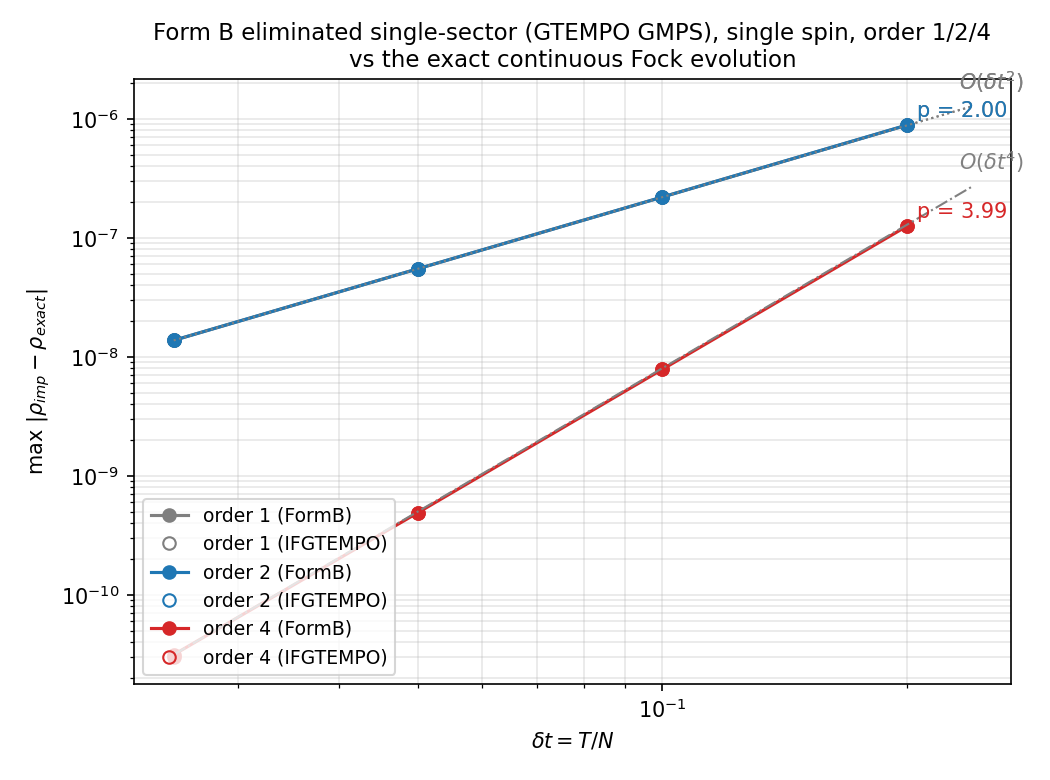
\includegraphics[width=0.86\textwidth]{../results/formb_scaling_single.png}
\caption{单自旋（$T=0.4$，$\epsilon_d=0.7$，$M=1$）：实线为 FormB
（GTEMPO GMPS 消元装配），空心点为 IFGTEMPO 两扇区 GMPS（同一离散链的
权威实现）——两者逐位重合。灰色参考线标 $O(\delta t^2)$/$O(\delta t^4)$。}
\label{fig:scaling-single}
\end{figure}

\begin{figure}[htbp]
\centering
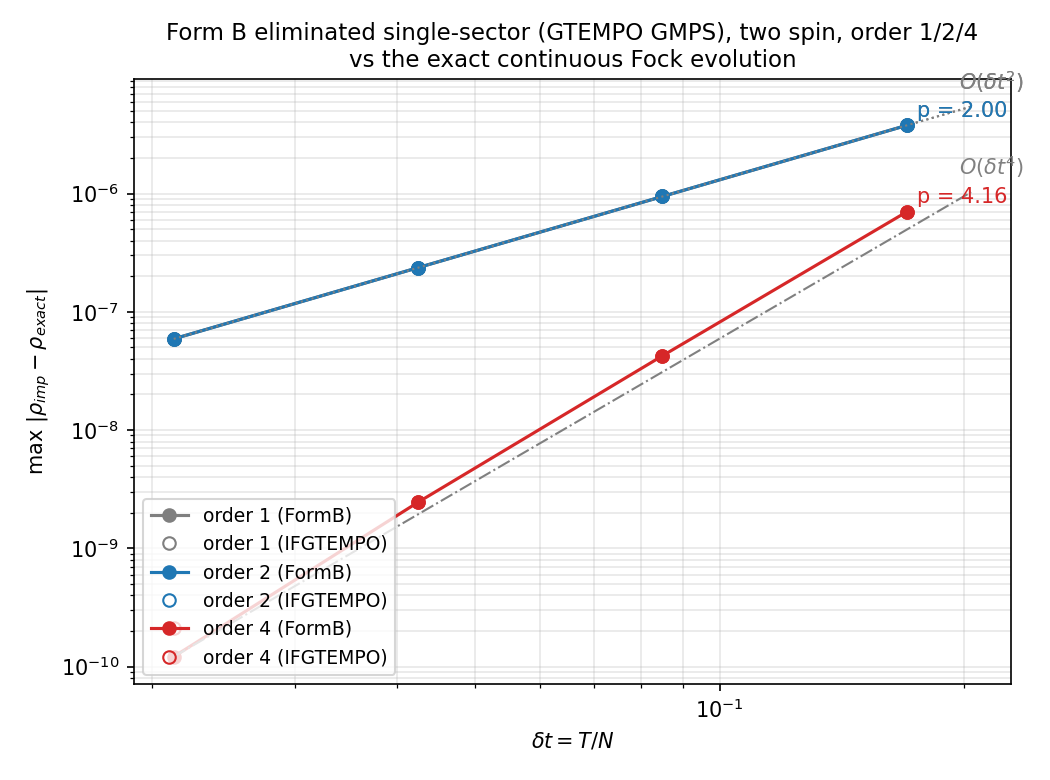
\includegraphics[width=0.86\textwidth]{../results/formb_scaling_twospin.png}
\caption{两自旋（$T=0.34$，$\epsilon=0.35/{-}0.22$，$U=1.0$，
$\rho_0=\mathrm{diag}(0,0.3,0.2,0.5)$，每自旋 $M=2$ bath）：
orders 1/2 全局二阶、order 4 四阶（比值 16.5/17.3，与 twosector
发表基准一致）。}
\label{fig:scaling-twospin}
\end{figure}

% ============================================================================
\appendix
\section{符号与约定速查}
% ============================================================================

\begin{center}
\begin{tabular}{ll}
\toprule
符号 & 含义 \\
\midrule
$a,\ab$（$x,\xb$） & IF（IMP）生成元；$\bar{\ }$ 为产生侧标签，非数值共轭 \\
slot $0,1,2,3$ & $(\ab^{+},a^{+},\ab^{-},a^{-})$；$\mathrm{flat}=4(t{-}1){+}\mathrm{slot}{+}1$ \\
$M_t$ & 接口交叉测度 $e^{-\ab_tx_t-\xb_ta_t}$（四个独立恒等之积） \\
$\Deff[\lambda,\lambda']$ & $-\tfrac12(G^{-1}[i,k]-G^{-1}[k,i])$，$\lambda{<}\lambda'$ 按 site 序 \\
$\nu\Pf(G)$ & bath 归一化 $\times$ IF Gaussian 的 Pfaffian \\
反测度 $(1-x_t\xb_t)$ & 抵消 GTEMPO 隐式 resolution 对接口对的重复施加（系数 $-1$） \\
闭合 $(1+\xb^{+}x^{-})$ & 反周期迹边界（翻转并入符号，系数 $+1$） \\
\bottomrule
\end{tabular}
\end{center}

\end{document}
